\documentclass{beamer}
%Information to be included in the title page:

\usepackage{csvsimple}
\usepackage{graphicx}
\graphicspath{ {./files/} } % Path relative to the main .tex file 

\usetheme{Berlin}
%\usecolortheme{dolphin}


\title{Regressione Lineare e Anova}

\subtitle{Progetto di Inferenza Statistica}

\author{T. Bucci, G. Corbo, D. Fabroni}

\institute{Politecnico di Milano}

\date{Luglio 2021}





\begin{document}

\frame{\titlepage}

\begin{frame}
    \frametitle{Table of Contents}
    \tableofcontents
\end{frame}

\section{Presentazione del dataset}
\begin{frame}
    \frametitle{Scelta del dataset: scoliosi}
    Fonte: Lichman, M. (2013). UCI Machine Learning Repository [\texttt{http://archive.ics.uci.edu/ml}]. Irvine, CA: University of California, School of Information and Computer Science
    %\footnote{\texttt{https://www.kaggle.com/uciml/biomechanical-features-of-orthopedic-patients?select=column_3C_weka.csv}}
\end{frame}


\begin{frame}
    \frametitle{Covariate presenti}
    \begin{itemize}
        \item pelvic incidence (continua)
        \item pelvic tilt (continua)
        \item lumbar lordosis angle (continua)
        \item sacral slope (continua)
        \item pelvic radius (continua)
        \item grade of spondylolisthesis (categorica)
    \end{itemize}
    con $310$ osservazioni.
\end{frame}


\section{Obiettivo}
\begin{frame}
    Vogliamo fare una regressione su misurazioni fisiche della zona pelvica...
    \begin{center}
        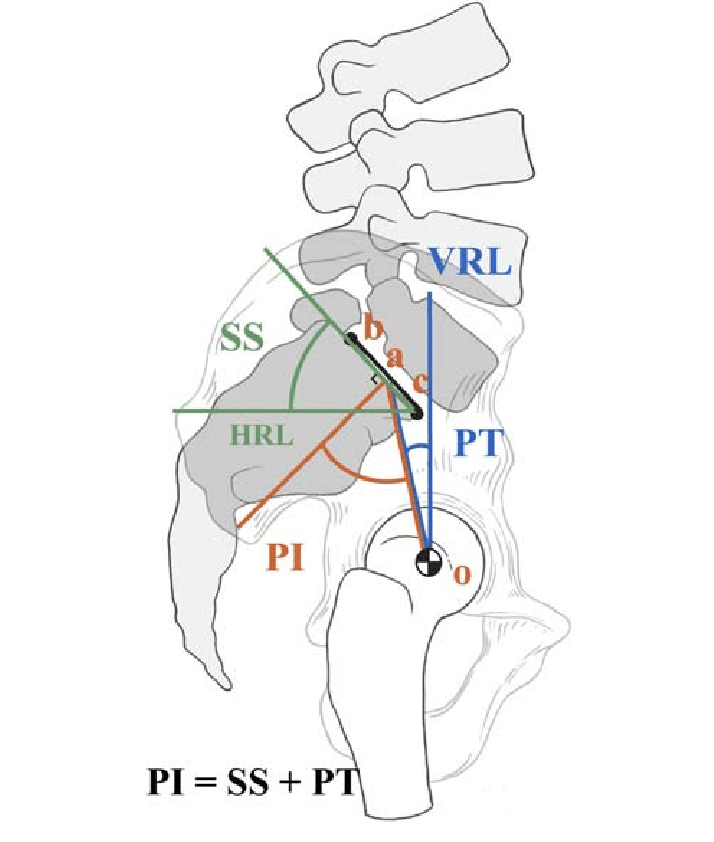
\includegraphics[width=0.35\textwidth]{bacino.png}
    \end{center}
\end{frame}


\begin{frame}
    ... per poter stimare il \textbf{lumbar lordosis angle}, un parametro che riguarda la sezione medio-bassa della schiena.
    \begin{center}
        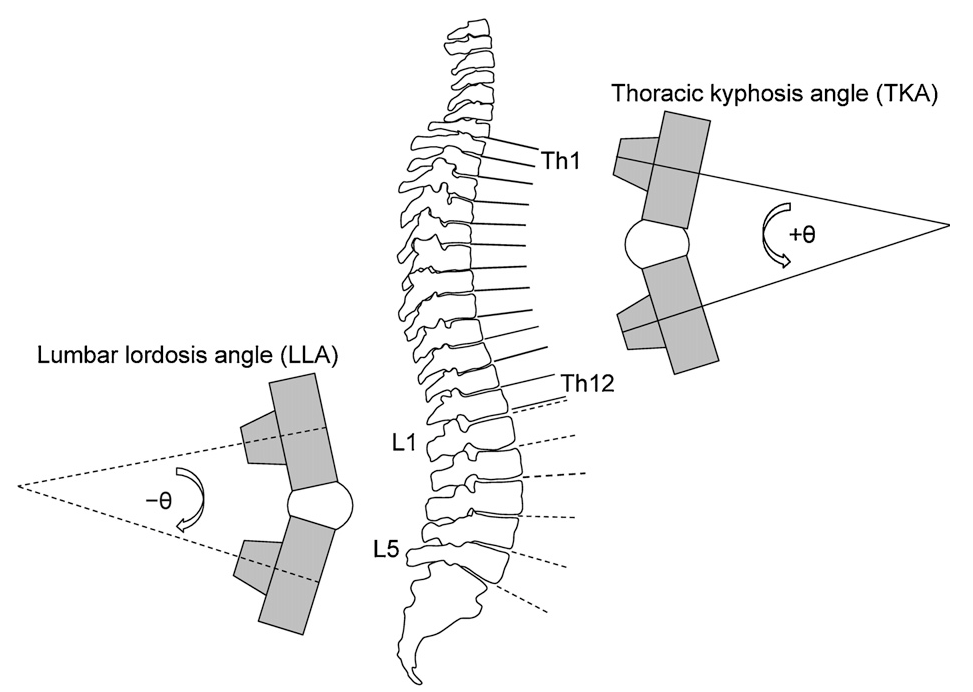
\includegraphics[width=0.5\textwidth]{lla.png}
    \end{center}
\end{frame}

\begin{frame}
    Vantaggi di questo approccio
    \begin{itemize}
        \item Poter prevedere una caratteristica della schiena senza fare una radiografia completa della schiena
        \item Risparmio di costi della radiografia
        \item Riduzione della quantità di raggi X a cui il paziente è esposto
    \end{itemize}
\end{frame}








\begin{frame}
	\textit{Pelvic tilt and sacral slope are two angles directly correlated with the pelvic incidence angle. The angle of incidence is the algebraic sum of two angles: pelvic tilt (PT) and sacral slope (SS)}\footnote{https://www.ncbi.nlm.nih.gov/pmc/articles/PMC3175921/}
\end{frame}





\begin{frame}
    \frametitle{Sample frame title}

    In this slide, some important text will be
    \alert{highlighted} because it's important.
    Please, don't abuse it.

    \begin{block}{Remark}
        Sample text
    \end{block}

    \begin{alertblock}{Important theorem}
        Sample text in red box
    \end{alertblock}

    \begin{examples}
        Sample text in green box. The title of the block is ``Examples".
    \end{examples}
\end{frame}


\end{document}